\documentclass[final]{beamer}

% -------------------------------------------------------------------------
% 1. PACKAGES & SETUP
% -------------------------------------------------------------------------

\usepackage[orientation=landscape,size=custom,width=91.44,height=60.96,scale=1.0]{beamerposter}

\setbeamersize{text margin left=0.25cm, text margin right=0.25cm}

\usepackage[utf8]{inputenc}
\usepackage[T1]{fontenc}
\usefonttheme{professionalfonts}
\usepackage{mathpazo}

\setlength{\parindent}{0pt}
\setlength{\parskip}{1pt}

\usepackage{xcolor}
\usepackage{graphicx}
\usepackage{grffile}
\graphicspath{{figures/}}
\usepackage{booktabs}
\usepackage{amsmath,amssymb}
\usepackage{url}
\usepackage{ragged2e}

\usepackage{tikz}
\usetikzlibrary{positioning,calc}

\usepackage{hyperref}

% -------------------------------------------------------------------------
% If the screenshot filenames below don't match yours, right-click each
% file in Overleaf's file tree to check the exact name and update below.
% -------------------------------------------------------------------------

% -------------------------------------------------------------------------
% 2. THEME & COLORS
% -------------------------------------------------------------------------

\definecolor{cardinalred}{RGB}{140,21,21}
\definecolor{coolgray}{RGB}{77,79,83}

\setbeamercolor{structure}{fg=cardinalred}
\setbeamercolor{title}{fg=white,bg=cardinalred}
\setbeamercolor{block title}{fg=white,bg=cardinalred}
\setbeamercolor{block body}{fg=black,bg=white}
\setbeamercolor{separation line}{bg=cardinalred}

\setbeamertemplate{block begin}{
  \vskip.5ex
  \begin{beamercolorbox}[leftskip=1cm,colsep*=.5ex]{block title}%
    \usebeamerfont*{block title}\insertblocktitle
  \end{beamercolorbox}%
  {\ifbeamercolorempty[bg]{block body}{}{\nointerlineskip\vskip-0.5pt}}%
  \usebeamerfont{block body}%
  \begin{beamercolorbox}[colsep*=.5ex,sep=.5ex,vmode]{block body}%
    \ifbeamercolorempty[bg]{block body}{\vskip-.25ex}{\vskip-.75ex}\vbox{}%
  \justifying
}
\setbeamertemplate{block end}{
  \end{beamercolorbox}
}

\setlength{\columnsep}{0.5cm}
\setlength{\columnseprule}{0.7pt}

\setbeamertemplate{itemize item}{\small\raise1.25pt\hbox{$\blacktriangleright$}}
\setbeamertemplate{itemize subitem}{\tiny\raise1.5pt\hbox{$\blacktriangleright$}}
\setbeamertemplate{itemize subsubitem}{\tiny\raise1.5pt\hbox{$\blacktriangleright$}}

\setbeamercolor{itemize item}{fg=cardinalred}
\setbeamercolor{itemize subitem}{fg=cardinalred}
\setbeamercolor{itemize subsubitem}{fg=cardinalred}

\setbeamertemplate{footline}{}
\setbeamertemplate{headline}{}
\setbeamertemplate{navigation symbols}{}
\setlength{\parskip}{2pt}

% -------------------------------------------------------------------------
% 3. METADATA
% -------------------------------------------------------------------------

\title{Aligning Physics Video Generation with Human Preferences\\via Reinforcement Learning}
\author{Hiva Mohammadzadeh \quad Pranav Kakhandiki \quad Douglas Kwok}
\institute{CS234: Reinforcement Learning, Stanford University}

\begin{document}

\begin{frame}[t,plain]
\begin{minipage}[t][0.98\textheight]{\textwidth}

% -------------------- Title bar --------------------
\begin{columns}[t,onlytextwidth]
  \begin{column}{\textwidth}
    \centering
    \vspace{-0.02cm}
    \begin{beamercolorbox}[wd=\textwidth,center,rounded=true,shadow=false]{title}
      \vspace{0.05cm}
      {\LARGE \textbf{\inserttitle}\par}
      \vspace{0.15cm}
      {\Large \insertauthor\par}
      \vspace{0.15cm}
      {\large \insertinstitute\par}
      \vspace{0.2cm}
    \end{beamercolorbox}
    \vspace{0.15cm}
  \end{column}
\end{columns}

% ======================== COLUMNS ===========================
\begin{columns}[t,onlytextwidth]

% ============================================================
% LEFT COLUMN
% ============================================================
\begin{column}{0.29\textwidth}

  \begin{block}{Introduction \& Motivation}
    \begin{itemize}
      \item Text-to-video diffusion models frequently violate
            \textbf{physical laws}---balls that float, pendulums
            that speed up, objects that ignore gravity.
      \item Standard denoising objectives do not encode physics priors.
      \item \textbf{Key insight}: RLHF and DPO can align video
            generators with human judgments of physical realism.
      \item \textbf{Goal}: End-to-end pipeline that
      \begin{enumerate}
        \item[\textbf{1.}] Generates physics simulation videos,
        \item[\textbf{2.}] Collects human preference rankings,
        \item[\textbf{3.}] Trains a reward model on preferences,
        \item[\textbf{4.}] Fine-tunes the generator via RLHF/DPO.
      \end{enumerate}
    \end{itemize}
  \end{block}

  \vspace{0.08cm}

  \begin{block}{Data Collection Pipeline}
    \begin{itemize}
      \item \textbf{48 text prompts} across three physics categories
            (16 each): Free-Falling Objects, Swinging Pendulum,
            Inclined Planes.
      \item Each prompt $\to$ \textbf{8 videos} via
            \textbf{Wan2.2-T2V-14B} (different seeds)
            $= \mathbf{384}$ videos.
      \item Annotators rank 8 videos per prompt (1\,=\,best to
            8\,=\,worst) on \textbf{Physical Accuracy},
            \textbf{Temporal Consistency}, and
            \textbf{Realism of Motion}.
      \item $\binom{8}{2}\!\times\!48 = \mathbf{1344}$ pairwise
            preference samples; ties excluded.
    \end{itemize}

    \vspace{0.15cm}
    \centering
    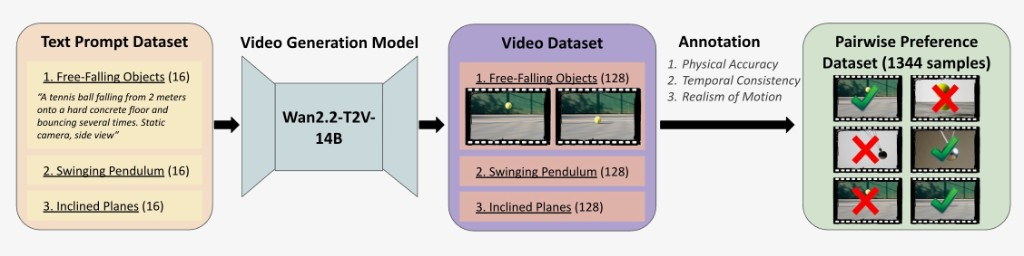
\includegraphics[width=\linewidth]{data_pipeline.png}
  \end{block}

  \vspace{0.08cm}

  \begin{block}{Experimental Setup}
    \begin{itemize}
      \item \textbf{Video Generation}: Wan2.2-T2V-14B via fal.ai;
            480p, 81~frames ($\sim$3.4\,s), guidance 3.5.
      \item \textbf{Reward Model}: Qwen3-VL-2B; LoRA $r\!=\!16$,
            $\alpha\!=\!32$; targets \texttt{to\_q/k/v/out}.
      \item \textbf{DPO}: $\beta\!=\!0.1$, lr$\,=\!10^{-6}$,
            batch 1, grad-accum 4, 10~epochs, Azure~ML~H100.
      \item \textbf{Features compared}: CLIP (frame-level),
            X-CLIP (video-level), Wan2.2 VAE (native latent).
      \item \textbf{Dataset}:
            \href{https://huggingface.co/datasets/hivamoh/wan22-physics-videos}
            {\texttt{hivamoh/wan22-physics-videos}}.
    \end{itemize}
  \end{block}

\end{column}

% ============================================================
% MIDDLE COLUMN
% ============================================================
\begin{column}{0.39\textwidth}

  \begin{block}{Reward Model Architecture}
    \begin{itemize}
      \item \textbf{Qwen3-VL-2B} backbone with \textbf{LoRA adapters}
            ($r\!=\!16$, $\alpha\!=\!32$) on vision encoder \&
            language model; base weights \textbf{frozen}.
            Trainable \textbf{linear head} $\to$ scalar reward~$r$.
      \item Trained with \textbf{Bradley--Terry} pairwise loss:\;
            $\mathcal{L}_{\text{BT}}
            = -\!\sum\log\sigma(r_i - r_j)$
    \end{itemize}

    \vspace{0.1cm}
    \centering
    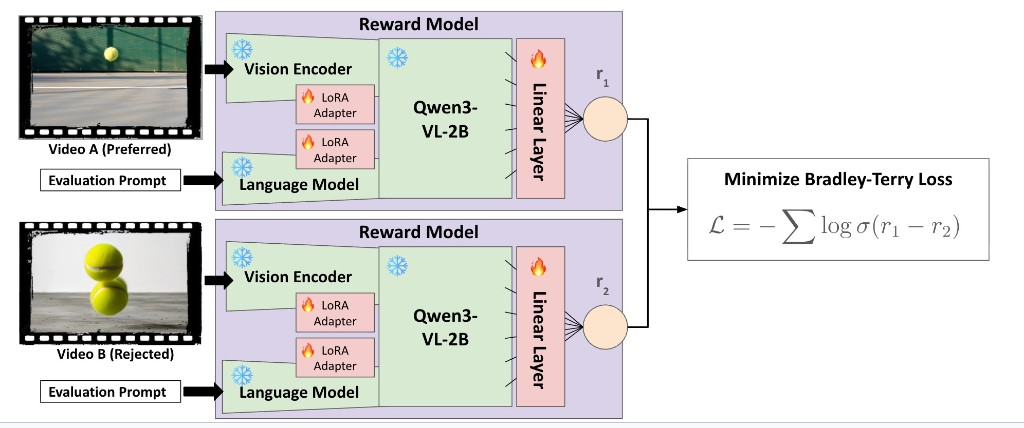
\includegraphics[width=0.85\linewidth]{reward_model.png}
  \end{block}

  \vspace{0.08cm}

  \begin{block}{Alignment Method 1: RLHF with PPO}
    \begin{itemize}
      \item Wan2.2 augmented with \textbf{trainable LoRA};
            base diffusion model \textbf{frozen}.
            Optimized via \textbf{PPO}:\;
            $\mathcal{L}_{\text{PPO}}
            \!=\! \sum [\min(z\hat{A},\,
            \text{clip}(z, 1\!-\!\epsilon, 1\!+\!\epsilon)\hat{A})]$,\;
            $z \!=\! \pi_{\text{cur}}/\pi_{\text{old}}$.
    \end{itemize}

    \vspace{0.1cm}
    \centering
    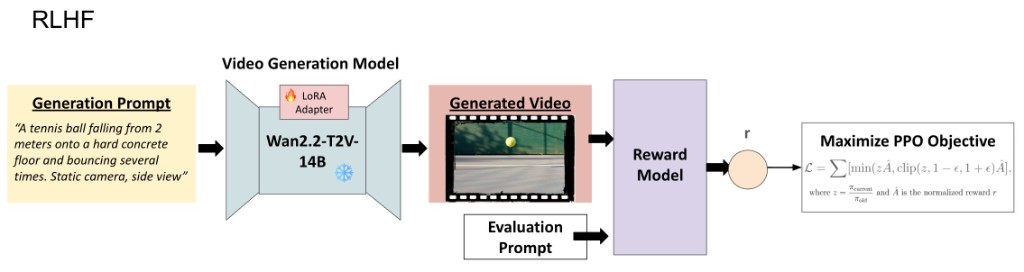
\includegraphics[width=0.85\linewidth]{rlhf_pipeline.png}
  \end{block}

  \vspace{0.08cm}

  \begin{block}{Alignment Method 2: DPO Fine-tuning}
    \begin{itemize}
      \item \textbf{No reward model} at training time;
            implicit reward = negative denoising MSE.
            Frozen copy = reference $\pi_{\text{ref}}$.\\[2pt]
            $\mathcal{L}_{\text{DPO}}
            \!=\! -\!\sum\log\sigma\!\bigl(
            \beta\log\frac{\pi_\theta(y^+|x)}{\pi_{\text{ref}}(y^+|x)}
            - \beta\log\frac{\pi_\theta(y^-|x)}{\pi_{\text{ref}}(y^-|x)}
            \bigr)$
    \end{itemize}

    \vspace{0.1cm}
    \centering
    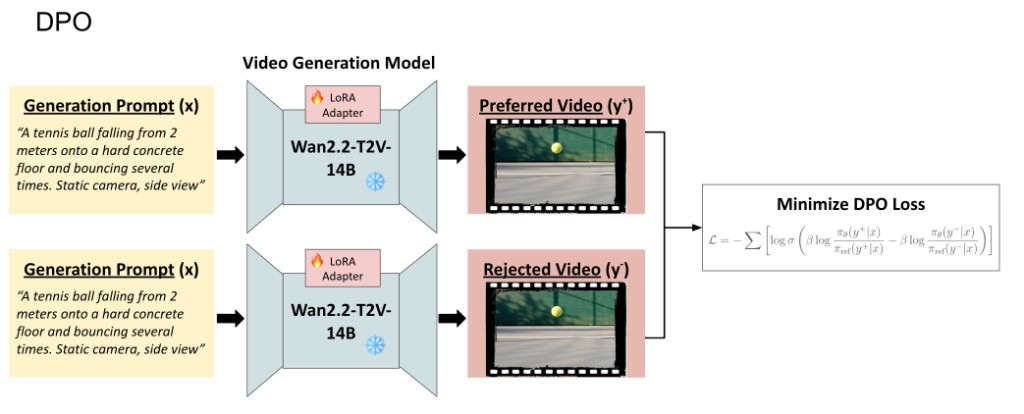
\includegraphics[width=0.85\linewidth]{dpo_pipeline.png}
  \end{block}

\end{column}

% ============================================================
% RIGHT COLUMN
% ============================================================
\begin{column}{0.29\textwidth}

  \begin{block}{Results: Reward Model}
    \centering
    \vspace{0.1cm}
    \setlength{\tabcolsep}{5pt}
    \renewcommand{\arraystretch}{1.25}
    \resizebox{0.95\linewidth}{!}{%
    \begin{tabular}{@{}lccc@{}}
      \toprule
      \textbf{Feature Extractor}
        & \textbf{BT Acc (\%)}
        & \textbf{DPO Acc (\%)}
        & \textbf{Kendall $\tau$} \\
      \midrule
      Random Baseline  & 50.0 & 50.0 & 0.00 \\
      CLIP             & 76.2 & 73.8 & 0.41 \\
      X-CLIP           & 80.5 & 78.1 & 0.52 \\
      \textbf{VAE Latent (Wan2.2)} & \textbf{83.4} & \textbf{81.2} & \textbf{0.59} \\
      \bottomrule
    \end{tabular}%
    }

    \vspace{0.3cm}

    \setlength{\tabcolsep}{5pt}
    \renewcommand{\arraystretch}{1.25}
    \resizebox{0.95\linewidth}{!}{%
    \begin{tabular}{@{}lcc@{}}
      \toprule
      \textbf{DPO Fine-tuning}
        & \textbf{Pref.\ Acc (\%)}
        & \textbf{Train Time} \\
      \midrule
      Before (base Wan2.2) & 50.0  & ---   \\
      After (LoRA-tuned)   & 72.4  & $\sim$3\,h (H100) \\
      \bottomrule
    \end{tabular}%
    }

    \vspace{0.15cm}
    {\small Pref.\ accuracy = fraction where policy favors the
    human-preferred video.}
  \end{block}

  \vspace{0.08cm}

  \begin{block}{Key Findings}
    \begin{itemize}
      \item \textbf{VAE latent features outperform CLIP/X-CLIP}
            for reward modeling---no feature mismatch with the
            generator's native latent space.
      \item The \textbf{same DPO loss} from standard RL
            (CS234 \texttt{run\_dpo.py}) transfers to diffusion
            models by using denoising MSE as implicit
            log-probability.
      \item \textbf{LoRA} enables fine-tuning the 14B-param Wan2.2
            with $<$24\,GB VRAM ($\sim$0.1\% of parameters).
      \item \textbf{Physics-specific prompts} are critical:
            ranking quality degrades when mixing physical and
            non-physical content.
    \end{itemize}
  \end{block}

  \vspace{0.08cm}

  \begin{block}{Conclusions \& Future Work}
    \textbf{Contributions:}
    \begin{itemize}
      \item End-to-end pipeline: video generation $\to$
            human preferences $\to$ reward model $\to$ fine-tuning.
      \item First application of RLHF and DPO to physics-focused
            T2V generation with Wan2.2.
      \item Systematic comparison of feature extractors for
            video reward modeling.
    \end{itemize}

    \vspace{0.15cm}
    \textbf{Future Directions:}
    \begin{itemize}
      \item \textbf{Multi-aspect rewards}: separate physics,
            visual quality, and motion scores.
      \item \textbf{Iterative DPO}: generate $\to$ rank $\to$
            retrain in closed-loop cycles.
      \item \textbf{Model distillation}: compress 14B model
            into a smaller, deployable variant.
      \item \textbf{Broader physics}: fluid dynamics,
            collisions, deformable objects.
    \end{itemize}
  \end{block}

\end{column}

\end{columns}

% ---------- overlay logos (uncomment when you have logo files) -----------
% \begin{tikzpicture}[remember picture,overlay]
%   \node[anchor=north east, xshift=-0.5cm, yshift=-0.3cm]
%     at (current page.north east) {%
%       \includegraphics[height=3cm]{stanford.png}%
%     };
%   \node[anchor=north west, xshift=0.5cm, yshift=-0.3cm]
%     at (current page.north west) {%
%       \includegraphics[height=3cm]{CS329A.pdf}%
%     };
% \end{tikzpicture}

\end{minipage}
\end{frame}

\end{document}
